%\documentclass[handout]{beamer}
\documentclass{beamer}
\usetheme{default}
\usepackage{amsmath}
\usepackage{amssymb}
\usepackage{tikz}  
\usepackage{xcolor}
\newcommand{\Z}{\mathbb{Z}}
\newcommand{\N}{\mathbb{N}}
\newcommand{\F}{\mathbb{F}}

\title{The AES in a nutshell}
\author{G. Averkov \\ Brandenburg University of Technology}
\begin{document}
\begin{frame}[plain]
    \maketitle
\end{frame}

\begin{frame}{High-level idea} 
	The AES is done over the field $F = \F_{256}$, realized as $F  = \Z_2 / g$ with $g = t^8 + t^4 + t^3 + t +1$. 
	The  field $F$ is an $8$-dimensional vector space over $\Z_2$. So, $F$ can be identified with $\Z_2^{8}$. The AES encrypts a list of $16$ elements of $F$. So, we can view the encryption map as a map $E_k : F^{16} \to F^{16}$ but also, in view of the identification, as a map $E_k : \Z_2^{128} \to \Z_2^{128}$. 
\end{frame} 

\begin{frame}
The incentive behind AES is to provide a map $E_k(x)$ that is highly non-linear in both $k$ and $x$. Remember that linearity and non-linearity is introduced with respect to a field: so, in our case, we could mean it in the sense of the field $\Z_2$ and in the sense of the field  $F$. The AES encoding map is built up of a sequence of operations that linear/affine and non-linear. Alternating between linear and non-linear operations,  within the AES, one makes a complicated non-linear map. 
\end{frame} 


\begin{frame}{The non-linear function on which AES relies} 
	One has $x^{|F|} = x$ for every $x \in F$, which follows from Lagrange's theorem. So, raising to the power $|F|$ is a linear map. Thus raising to the power $x^{|F|-1}$ is a map that is equal to $1$ on $x \in F \setminus \{0\}$ and equal to $0$ on $x=0$. This one is not invertible and not complicated (so, no good for the encryption). But raising to the power $|F|-2$ is pretty much the same as the inversion of $x$ (it gives $x^{-1}$ for $x \ne 0$ and $0$ for $x =0$). Raising to the power $|F|-2$ can be implemented efficiently (because the inversion in $F$ can be implemented efficiently). The map is not only highly non-linear with respect to $F$, but also with respect to $\Z_2$. 
\end{frame} 


\begin{frame}{Non-linearity of inversion in a field - Example~1} 
	If we had $F = \Z_2[t] / (t^3 + t+1)$ with $\alpha$ being the coset of $t$ modulo $t^3 + t+1$, then 
	\[
		x = x_0 + x_1 \alpha  + x_2 \alpha^2 \leftrightarrow (x_0,\,x_1,\,x_2)
	\] raised to the power $|F|-2 = 6$ would be 
	\begin{align*} 
		x^6 & = x_0 + x_1 + x_2 + x_1 x_2 + (x_0 x_1 + x_2) \alpha + (x_0 x_2 + x_1 + x_2) \alpha^2
		\\ & \leftrightarrow (x_0 + x_1 + x_2 + x_1 x_2, \, x_0 x_1 + x_2, \, x_0 x_2 + x_1 + x_2). 
	\end{align*} 
	The dependence on $x_0, x_1, x_2 \in \Z_2$ is non-linear. The dependence of $x^{|F|-2}$ on $x_0,\ldots,x_{n-1}$ gets even more non-linear when $F$ the dimension $n$ of $F$ over $\Z_2$ gets even higher. 
\end{frame} 

\begin{frame}{Non-linearity of inversion in a field - Example~2}
	If we had $F = \Z_2[t] / (t^4 + t+1)$ with $\alpha$ being the coset of $t$ modulo $t^4 + t+1$, then 
	\begin{align*} 
		 & x^4 = (x_0  + x_1 \alpha + x_2 \alpha^2 + x_3 \alpha^3)^{14}  
		\\  \leftrightarrow ( & x_{0} x_{1} x_{2} + x_{1} x_{2} x_{3} + x_{0} x_{2} + x_{1} x_{2} + x_{0} + x_{1} + x_{2} + x_{3},
		\\ & x_{0} x_{1} x_{3} + x_{0} x_{1} + x_{0} x_{2} + x_{1} x_{2} + x_{1} x_{3} + x_{3},
		\\ & x_{0} x_{2} x_{3} + x_{0} x_{1} + x_{0} x_{2} + x_{0} x_{3} + x_{2} + x_{3}, 
		\\ & x_{1} x_{2} x_{3} + x_{0} x_{3} + x_{1} x_{3} + x_{2} x_{3} + x_{1} + x_{2} + x_{3} )
	\end{align*} 
\end{frame} 

\newcommand{\byte}{\square\square\square\square\square\square\square\square} 
\begin{frame}{}
	The AES pipelines the initial data (the message), consisting of $8 \cdot 4 \cdot 4 = 128$ bits, through a sequence of transformations that jumble and reshuffle the data in each stage in a rather complicated way. The data is a $4 \times 4$ table ($=$ a matrix), with each entry being an element of $F$, which corresponds to $8$ bits of information. Imagine writing bits into the squares of the following table: 
	\[ \scriptsize 
	\begin{bmatrix} 
		\byte & \byte & \byte & \byte \\
		\byte & \byte & \byte & \byte \\
		\byte & \byte & \byte & \byte \\
		\byte & \byte & \byte & \byte 		
	\end{bmatrix} 
	\]
\end{frame} 

\begin{frame}{}
	\begin{enumerate}[<+->]
	\item	One type of the transformation is  localized to the elements of $F$, and so it changes each  of the $16$ entries of the table independently of each other. So, this transformation is local, in the sense that it jumbles the $8$-bit groups independently of each other. This transformation is highly non-linear. 
	\item Another type of transformation reshuffles the bits within each of the $4$ rows independently. 
	\item Yet another transformation jumbles the bits within each of the $4$ columns independently. This transformation is affine. 
	\end{enumerate} 
\end{frame} 

\begin{frame} 
		When all three types of transformations are applied successively, one makes sure that there is a lot of non-linearity in the process of encryption and that each of the $128$ bits of the plain text affects each of the $128$ bits of the cipher text and, vice versa, that each fo the $128$ of the cipher text is affected in a complicated manner by each fo the $128$ bits of the plain text. 
\end{frame} 

\begin{frame}
	It's like doing a fondue. Fondue is a liquid cheese in a pot made in Switzerland. So, the AES is a fondue done out of 128 bits. When you do the fondue, you stir the cheese in a pot. Our pot is consisting of $4 \times 4$ spots, each having $8$ bits. There are several ways to stir. You can stir each of the $16$ $8$-bit groups. You could stir row-wise, each of the $4$ rows, and you can stir column-wise, each of the $4$ columns. The AES encryption of a message is prepared by combining all these ways to stir. 
\end{frame} 

\begin{frame} 
	The key of AES is $k \in F^{4 \times 4}$ and, so it is also given by $128$ bits. The AES has a procedure (to be described below) that associates to $k$ a sequence of the so-called round keys $k^{(0)},\ldots,k^{(10)} \in F^{4 \times 4}$, calculated iteratively starting with $k^{(0)} = k$. 
	
	\vspace{3mm}
	
	The plain text message $M = (m_{i,j})_{i,j=0,\ldots,3} \in F^{4 \times 4}$ undergoes a sequence of transformations, carried out iteratively and producing a sequence $M^{(0)},\ldots,M^{(10)} \in F^{4 \times 4}$ with the final result $M^{(10)}$ being the cyphertext for $M$. 
\end{frame} 

\newcommand{\SB}{\operatorname{SB}}
\begin{frame}{SubBytes} 
	We introduce the transformation \emph{SubBytes}
	$\SB : F^{4 \times 4} \to F^{4 \times 4}$ that acts on $ M = (m_{i,j})_{i,j=0,\ldots,3} \in F^{4 \times 4}$ by 
	\[
		\SB(M) = \biggl( T( {m_{i,j}}^{254}) + 1 + \alpha + \alpha^5 + \alpha^6 \biggr)_{i,j=0,\ldots,3},
	\]
	where $T : F \to F$ is the $\Z_2$-linear transformation 
	\[
		T( x_0 \alpha +\cdots + x_7 \alpha^7) = y_0 \alpha + \cdots + y_7 \alpha^7
	\] 
	given by...
\end{frame} 

\begin{frame}{SubBytes matrix} 
		\[
	\begin{bmatrix} y_0 \\ y_1 \\ y_2 \\ y_3 \\ y_4 \\ y_5 \\ y_6 \\ y_7 \end{bmatrix} = \begin{bmatrix} 1 & 0 & 0 & 0 & 1 & 1 & 1 & 1 
	\\ 1 & 1 & 0 & 0 & 0 & 1 & 1 & 1 
\\ 1 & 1 & 1 & 0 & 0 & 0 & 1 & 1 
\\ 1 & 1 & 1 & 1 & 0 & 0 & 0 & 1 
\\ 1 & 1 & 1 & 1 & 1 & 0 & 0 & 0 
\\ 0 & 1 & 1 & 1 & 1 & 1 & 0 & 0 
\\ 0 & 0 & 1 & 1 & 1 & 1 & 1 & 0 
\\ 0 & 0 & 0 & 1 & 1  & 1 & 1 & 1 \end{bmatrix} \begin{bmatrix} x_0 \\ x_1 \\ x_2 \\ x_3 \\ x_4 \\ x_5 \\ x_6 \\ x_7 \end{bmatrix} 
	\]
\end{frame} 

\begin{frame}{SubBytes matrix, continued} 
	Equivalently, the dependence of $y$ on $x$ is 
	\[
		y _i = x_i + x_{i-1} + x_{i-2} + x_{i-3} + x_{i-4},
	\] 
	with the indexing modulo $8$. 
	
	$\SB$ is an invertible transformation, because raising to the power $254$ is invertible, and there is a one-to-one correspondence $x \leftrightarrow y$, as \ldots
\end{frame} 

\begin{frame}
	\begin{center} 
	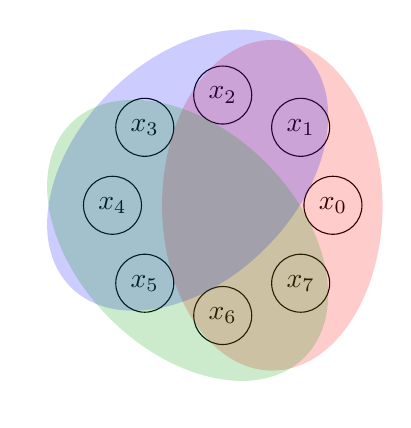
\begin{tikzpicture}[scale=0.7]
		 \foreach \i in {0,1,...,7} {
			\node[circle, draw, minimum size=3mm] (x\i) at ({360/8 * \i}: 2) {$x_\i$};
		}
		\fill[color=red,very thick,opacity=0.2] (0.9,0) ellipse (2cm and 3cm) ;
		\fill[color=blue,very thick,rotate=135,opacity=0.2] (0.9,0) ellipse (2cm and 3cm) ;
		\fill[color=green!60!black,very thick,rotate=-135,opacity=0.2] (0.9,0) ellipse (2cm and 3cm) ;
	\end{tikzpicture} 
	\end{center} 
	\[
		x_0 = y_2 + y_5 + y_7
	\]
	Generally, 
	\[
		x_i = y_{i+2} + y_{i+5} + y_{i+7}.
	\]
\end{frame} 



%\newcommand{\aux}[1]{\mathbb{#1}}

\begin{frame}{ShiftRows}
	\[
		(m_{i,j})_{i,j=0,\ldots,3} \qquad \xrightarrow{ShiftRows} \qquad ( m_{i,j - i} )_{i,j=0,\ldots,3}. 
	\]
	\vspace{3mm}
	\begin{center} 
		\tiny
	\begin{tabular}{|cccc|}
			\hline 
		\colorbox{red!30}{$m_{0,0}$} & \colorbox{green!30}{$m_{0,1}$} & \colorbox{orange!30}{$m_{0,2}$}  & \colorbox{blue!30}{$m_{0,3}$} 
\\ \hline 
		\colorbox{red!30}{$m_{1,0}$} & \colorbox{green!30}{$m_{1,1}$} & \colorbox{orange!30}{$m_{1,2}$}  & \colorbox{blue!30}{$m_{1,3}$} 
\\ \hline 
		\colorbox{red!30}{$m_{2,0}$} & \colorbox{green!30}{$m_{2,1}$} & \colorbox{orange!30}{$m_{2,2}$}  & \colorbox{blue!30}{$m_{0,3}$} 
\\ \hline 
		\colorbox{red!30}{$m_{3,0}$} & \colorbox{green!30}{$m_{3,1}$} & \colorbox{orange!30}{$m_{3,2}$}  & \colorbox{blue!30}{$m_{3,3}$} 
\\ \hline 
	\end{tabular} 
	$\xrightarrow{ShiftRows}$
	\begin{tabular}{|cccc|}
			\hline 
			\colorbox{red!30}{$m_{0,0}$} & \colorbox{green!30}{$m_{0,1}$} & \colorbox{orange!30}{$m_{0,2}$}  & \colorbox{blue!30}{$m_{0,3}$} 
			\\ \hline 
			\colorbox{green!30}{$m_{1,1}$} & \colorbox{orange!30}{$m_{1,2}$} & \colorbox{blue!30}{$m_{1,3}$} & \colorbox{red!30}{$m_{1,0}$}   
			\\ \hline 
			\colorbox{orange!30}{$m_{2,2}$}   & \colorbox{blue!30}{$m_{2,3}$} & \colorbox{red!30}{$m_{2,0}$} & \colorbox{green!30}{$m_{2,1}$}  
			\\ \hline 
		 \colorbox{blue!30}{$m_{3,3}$}  & \colorbox{red!30}{$m_{3,0}$}   & \colorbox{green!30}{$m_{3,1}$} & \colorbox{orange!30}{$m_{3,2}$} \\ \hline
	\end{tabular} 
	\end{center} 
\end{frame} 

\begin{frame}{MixColumns} 
	\[
		M \xrightarrow{MixColumns}T M
	\]
	with 
	\[ 
			T = \begin{bmatrix} \alpha & 1 + \alpha & 1 & 1
		\\	1 & \alpha & 1 + \alpha & 1 
		\\ 1 & 1 & \alpha & 1+\alpha
	\\ 1 + \alpha & 1 & 1 & \alpha \end{bmatrix}.
	\]
	MixColumns transforms each column of $M$ independently. Let's see how this transformation works. 
\end{frame} 

\begin{frame}{Interpretation of MixColumns} 
	\begin{align*}
		& f := m_0 + m_1 u + m_2 u^2 + m_3 u^3 \in F[u]
		\\ & \mapsto 
		\\  & (\alpha + u + u^2 + (1+\alpha) u^3) f \bmod (u^4 +1 ). 
	\end{align*} 
	This corresponds to a linear transformation on the ring $G = F[u] / (u^4 + 1)$. tt is invertible, because 
	$(u^4+1) = (u+1)^4$ in $F[u]$. This shows that $a(u) :=\alpha + u + u^2 + (1+\alpha) u^3$ and $u^4+1$ are relatively prime because $a(1) = \alpha + 1 + 1 + (1+\alpha) = 1$. 
\end{frame} 

\begin{frame}{Round keys}  
	$k = (k[0],\ldots,k[3]) \in F^{4 \times 4} $. One generates
	\[
		(k[0],\ldots,k[39]) \in F^{4 \times 40}
	\]
	by the following rule for $i \ge 4$: 
	\[
		k[i] = \begin{cases} 
				k[i-4] + k[i-1], & i \ \text{is not divisible by} \ 4,
				\\ k[i-4] + \SB(k[i-1]) + s & i \ \text{divisible by} \ 4,
			\end{cases} 		
	\]
	where 
	\[
		s = \begin{bmatrix} \alpha^{i/4 - 1} \\ 0 \\ 0 \\ 0\end{bmatrix}. 
	\]
	The round keys are
	\[
		k^{(i)} = ( k[4 i], k[4i +1], k[4i+2], k[4i+3] ) \in F^{4 \times 4}.
	\]
\end{frame} 

\begin{frame}{AES keys} 
\begin{center} 
\includegraphics[width=3cm]{aes_keys.png}
\end{center} 
\end{frame} 

\begin{frame}{Encryption $(k,M) \mapsto M^{(10)}$} 
	\begin{itemize} 
		\item $M^{(0)} = k^{(0)} + M $
		\item $M^{(i)} = k^{(i)} + \operatorname{MixColumns} ( \operatorname{ShiftRows} (\operatorname{SubBytes} (M^{(i-1)})))$ for $i=1,\ldots,9$
		\item $M^{(10)}  = k^{(10)} + \operatorname{ShiftRows} ( \operatorname{SubBytes} (M^{(9)} )$ 
	\end{itemize} 
\end{frame} 

\end{document}
